\subsection{basic definitions}

\begin{frame}
\begin{center}
	\begin{restofframe}
		\begin{tikzpicture}
  \path[mindmap,concept color=black,text=white]
    node[concept] {\_\_\_\_\_ algebra}
    [clockwise from=0]
    child[concept color=green!50!black] {
      node[concept] {abstract}
      [counterclockwise from=-135]
      child { node[concept] {classes of algebraic structures} }
      child { node[concept] {monoids, groups, rings, fields, \ldots} }
%      child { node[concept] {monoids} }
%      child { node[concept] {semigroups} }
%      child { node[concept] {groups} }
%      child { node[concept] {rings} }
%      child { node[concept] {fields} }
%      child { node[concept] {all in between...} }
    }  
    child[concept color=blue] {
      node[concept] {elementary}
      [clockwise from=-30]
      child { node[concept] {formulas} }
      child { node[concept] {laws} }
      child { node[concept] {cartesian geometry} }   
    }
    child[concept color=red] {
     node[concept] {universal} 
     [clockwise from=-90]
          child { node[concept] {varieties, quasivarieties, elementary classes} }
          child { node[concept] {classes of classes of algebraic structures} }
    }
    child[concept color=orange] {
     node[concept] {categorical} 
     [clockwise from=-30]
	    child { node[concept] {objects} }
  	   %child { node[concept] {morphisms} }
  	    child { node[concept] {$(n,r)$-morphisms} }
	};
\end{tikzpicture}
	\end{restofframe}
\end{center}
\end{frame}

\begin{frame}
\frametitle{A quasi-hierarchy of algebraic theories}
	\begin{description}
		\item[Theory] :: domain of discourse
		\item[Elementary Algebra] :: equational reasoning in a particular algebra
		\item[Abstract Algebra] :: particular classes of algebras such as groups, rings, or fields
		\item[Universal algebra] :: classes of classes of algebras
		\item[Category theory] :: given a list of operations and axioms in universal algebra the corresponding algebras and homomorphisms between them can represent objects and morphisms in a category
	\end{description}
\end{frame}

\begin{frame}
\frametitle{category theory}
	\begin{center}
		
\includegraphics[scale=0.4]{fig/stacksproject.png}
	\end{center}
	\href{http://www.math.columbia.edu/algebraic_geometry/stacks-git/}{the stacks project ::}
	\url{http://www.math.columbia.edu/algebraic_geometry/stacks-git/}
\end{frame}

\begin{frame}
\iftoggle{thmsty}{
\begin{definition}
\label{definition-category}
}{}
A {\it category} $\mathcal{C}$ is:
\begin{enumerate}
\item A set of objects $\Ob(\mathcal{C})$.
\item For each pair $x, y \in \Ob(\mathcal{C})$ a set of morphisms
$\Mor_\mathcal{C}(x, y)$.
\item For each triple $x, y, z\in \Ob(\mathcal{C})$ a composition
map $ \Mor_\mathcal{C}(y, z) \times \Mor_\mathcal{C}(x, y)
\to \Mor_\mathcal{C}(x, z) $, denoted $(\phi, \psi) \mapsto
\phi \circ \psi$.
\end{enumerate}
Such that these constraints are satisfied:
\begin{enumerate}
\item For every element $x\in \Ob(\mathcal{C})$ there exists a
morphism $\text{id}_x\in \Mor_\mathcal{C}(x, x)$ such that
$\text{id}_x \circ \phi = \phi$ and $\psi \circ \text{id}_x = \psi $.
\item Composition is associative, i.e., $(\phi \circ \psi) \circ \chi =
\phi \circ ( \psi \circ \chi)$.
\end{enumerate}
\iftoggle{thmsty}{
\end{definition}
}
\end{frame}


\begin{frame}
\iftoggle{thmsty}{
\begin{definition}
\label{definition-functor}
}{}
A {\it functor} $F : \mathcal{A} \to \mathcal{B}$
between two categories $\mathcal{A}, \mathcal{B}$ is:
\begin{enumerate}
\item A map $F : \Ob(\mathcal{A}) \to \Ob(\mathcal{B})$.
\item For every $x, y \in \Ob(\mathcal{A})$ a map
$F : \Mor_\mathcal{A}(x, y) \to \Mor_\mathcal{B}(F(x), F(y))$,
denoted $\phi \mapsto F(\phi)$.
\end{enumerate}
These data should be compatible with composition and identity morphisms
in the following manner: $F(\phi \circ \psi) =
F(\phi) \circ F(\psi)$ for a composable pair $(\phi, \psi)$ of
morphisms of $\mathcal{A}$ and $F(\text{id}_x) = \text{id}_{F(x)}$.
\iftoggle{thmsty}{
\end{definition}
}
\end{frame}

\begin{frame}
\iftoggle{thmsty}{
\begin{definition}
\label{definition-transformation-functors}
}{}
Let $F, G : \mathcal{A} \to \mathcal{B}$ be functors.
A {\it natural transformation}, or a {\it morphism of functors}
$t : F \to G$, is a collection $\{t_x\}_{x\in \Ob(\mathcal{A})}$
such that
\begin{enumerate}
\item $t_x : F(x) \to G(x)$ is a morphism in the category $\mathcal{B}$, and
\item for every morphism $\phi : x \to y$ of $\mathcal{A}$ the following
diagram is commutative
$$
\xymatrix{
F(x) \ar[r]^{t_x} \ar[d]_{F(\phi)} & G(x) \ar[d]^{G(\phi)} \\
F(y) \ar[r]^{t_y} & G(y) }
$$
\end{enumerate}
\iftoggle{thmsty}{
\end{definition}
}
\end{frame}

\begin{frame}
%\frametitle{category theory}
	The diagram
	$$
	\xymatrix{
	\mathcal{A}
	\rtwocell^F_G{t}
	&
	\mathcal{B}
	}
	$$
	can be used to indicate that $t$ is a morphism (a natural transformation in particular) between functors $F$ and $G$.
\end{frame}

\iftoggle{longpres}{

\subsection{co products}

\begin{frame}
\iftoggle{thmsty}{
\begin{definition}
\label{definition-products}
}{}

Let $x, y\in \Ob(\mathcal{C})$,
A {\it product} of $x$ and $y$ is
an object $x \times y \in \Ob(\mathcal{C})$
together with morphisms
$p\in \Mor_{\mathcal C}(x \times y, x)$ and
$q\in\Mor_{\mathcal C}(x \times y, y)$ such
that the following universal property holds: for
any $w\in \Ob(\mathcal{C})$ and morphisms
$\alpha \in \Mor_{\mathcal C}(w, x)$ and
$\beta \in \Mor_\mathcal{C}(w, y)$
there is a unique
$\gamma\in \Mor_{\mathcal C}(w, x \times y)$ making
the diagram
$$
\xymatrix{
w \ar[rrrd]^\beta \ar@{-->}[rrd]_\gamma \ar[rrdd]_\alpha & & \\
& & x \times y \ar[d]_p \ar[r]_q & z \\
& & x &
}
$$
commute.
\iftoggle{thmsty}{
\end{definition}
}
\end{frame}

\begin{frame}
\iftoggle{thmsty}{
\begin{definition}
\label{definition-has-products-of-pairs}
}{}
We say the category $\mathcal{C}$ {\it has products of pairs
of objects} if a product $x \times y$
exists for any $x, y \in \Ob(\mathcal{C})$.
\iftoggle{thmsty}{
\end{definition}
}
\end{frame}

\begin{frame}
\iftoggle{thmsty}{
\begin{definition}
\label{definition-product-category}
}{}
Let $\mathcal{A}$, $\mathcal{B}$ be categories.
The {\it product category} is the category
$\mathcal{A} \times \mathcal{B}$ with
objects
$\Ob(\mathcal{A} \times \mathcal{B}) =
\Ob(\mathcal{A}) \times \Ob(\mathcal{B})$
and
$$
\Mor_{\mathcal{A} \times \mathcal{B}}((x, y), (x', y'))
:=
\Mor_\mathcal{A}(x, x')\times
\Mor_\mathcal{B}(y, y').
$$
Composition of morphisms is defined according to components.
\iftoggle{thmsty}{
\end{definition}
}
\end{frame}

\begin{frame}
\iftoggle{thmsty}{
\begin{definition}
\label{definition-coproducts}
}{}
Let $x, y \in \Ob(\mathcal{C})$,
A {\it coproduct}, or {\it amalgamated sum} of $x$ and $y$ is
an object $x \amalg y \in \Ob(\mathcal{C})$
together with morphisms
$i \in \Mor_{\mathcal C}(x, x \amalg y)$ and
$j \in \Mor_{\mathcal C}(y, x \amalg y)$ such
that the following universal property holds: for
any $w \in \Ob(\mathcal{C})$ and morphisms
$\alpha \in \Mor_{\mathcal C}(x, w)$ and
$\beta \in \Mor_\mathcal{C}(y, w)$
there is a unique
$\gamma \in \Mor_{\mathcal C}(x \amalg y, w)$ making
the diagram
$$
\xymatrix{
& y \ar[d]^j \ar[rrdd]^\beta \\
x \ar[r]^i \ar[rrrd]_\alpha & x \amalg y \ar@{-->}[rrd]^\gamma \\
& & & w
}
$$
commute.
\iftoggle{thmsty}{
\end{definition}
}
\end{frame}

\begin{frame}
\iftoggle{thmsty}{
\begin{definition}
\label{definition-has-coproducts-of-pairs}
}{}
We say the category $\mathcal{C}$ {\it has coproducts of pairs
of objects} if a coproduct $x \amalg y$
exists for any $x, y \in \Ob(\mathcal{C})$.
\iftoggle{thmsty}{
\end{definition}
}
\end{frame}

}{}


\subsection{co equalizers}

\begin{frame}
\iftoggle{thmsty}{
\begin{definition}
\label{definition-initial-final}
}{}
Let $\mathcal{C}$ be a category.
\begin{enumerate}
\item An object $x$ of the category $\mathcal{C}$ is called
an {\it initial} object if for every object $y$ of $\mathcal{C}$
there is exactly one morphism $x \to y$.
\item An object $x$ of the category $\mathcal{C}$ is called
a {\it final} object if for every object $y$ of $\mathcal{C}$
there is exactly one morphism $y \to x$.
\end{enumerate}
\iftoggle{thmsty}{
\end{definition}
}
\end{frame}

\begin{frame}
\noindent For example, in \textit{Sets} the empty set $\emptyset$ is the unique
initial object and any {\it singleton} set, a set with one element,
is a final object.
\end{frame}

\begin{frame}
\iftoggle{thmsty}{
\begin{definition}
\label{definition-equalizers}
}{}
Suppose that $X$, $Y$ are objects of a category $\mathcal{C}$
and that $a, b : X \to Y$ are morphisms. We say a morphism
$e : Z \to X$ is an {\it equalizer} for the pair $(a, b)$ if
$a \circ e = b \circ e$ and if $(Z, e)$ satisfies the following
universal property: For every morphism $t : W \to X$
in $\mathcal{C}$ such that $a \circ t = b \circ t$ there exists
a unique morphism $s : W \to Z$ such that $t = e \circ s$.
\iftoggle{thmsty}{
\end{definition}
}

\begin{displaymath}
\xymatrix{
X
\ar@<1ex>[r]^-{a} \ar@<-1ex>[r]_-{b}
&
Y \ar[r]^-{c} \ar[dr]_-{t}
&
Z \ar@{-->}[d]^-{s}\\
& & W
}
\end{displaymath}
\end{frame}

\begin{frame}
\begin{figure}
\noindent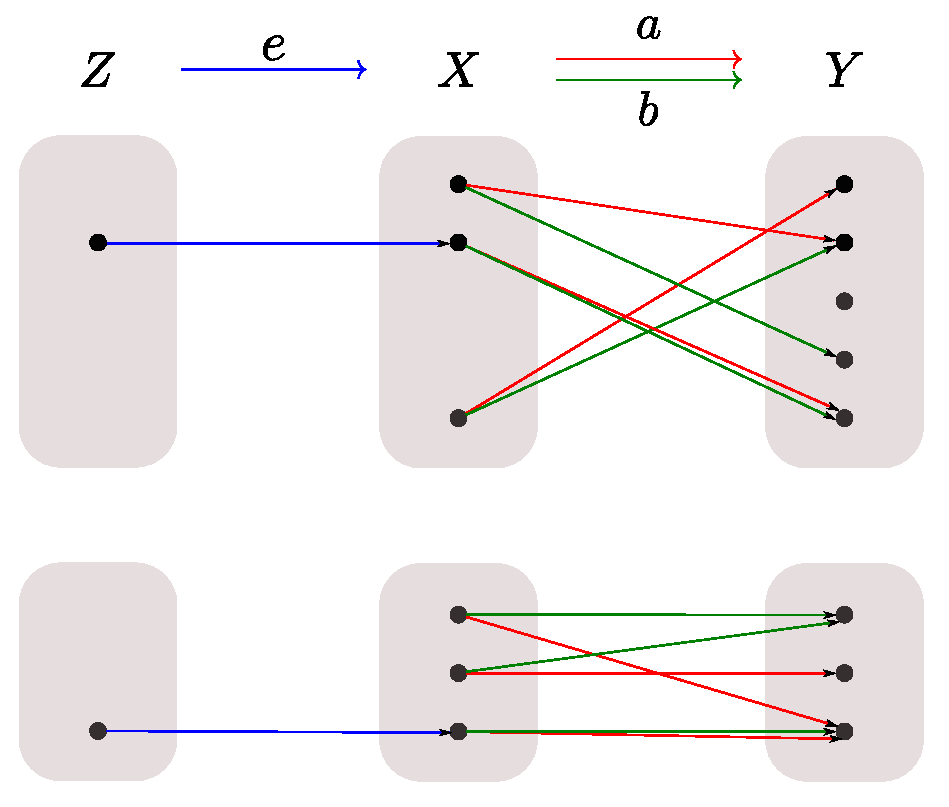
\includegraphics[width=0.8\framewidth]{fig/equalizer.pdf}
\caption{Examples of equalizers in the category of finite sets.}
\label{fig:equalizer}
\end{figure}
\end{frame}

\begin{frame}
\iftoggle{thmsty}{
\begin{definition}
\label{definition-coequalizers}
}{}
Suppose that $X$, $Y$ are objects of a category $\mathcal{C}$
and that $a, b : X \to Y$ are morphisms. We say a morphism
$c : Y \to Z$ is a {\it coequalizer} for the pair $(a, b)$ if
$c \circ a = c \circ b$ and if $(Z, c)$ satisfies the following
universal property: For every morphism $t : Y \to W$
in $\mathcal{C}$ such that $t \circ a = t \circ b$ there exists
a unique morphism $s : Z \to W$ such that $t = s \circ c$.
\iftoggle{thmsty}{
\end{definition}
}

\begin{displaymath}
\xymatrix{
Z \ar[r]^-{c}
&
X \ar@<1ex>[r]^-{a} \ar@<-1ex>[r]_-{b}
&
Y\\
W \ar@{-->}[u]^-{s} \ar[ur]_-{t} & &
}
\end{displaymath}
\end{frame}

\begin{frame}
\begin{figure}
\noindent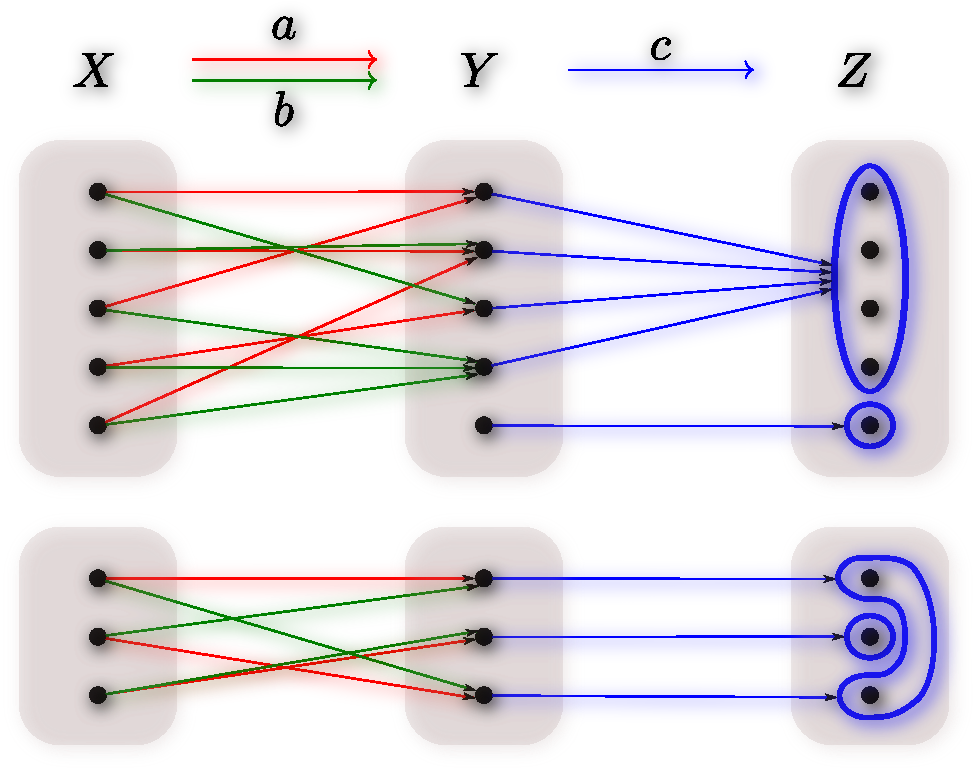
\includegraphics[width=0.8\framewidth]{fig/coequalizer.pdf}
\caption{Examples of coequalizers in the category of finite sets.}
\label{fig:coequalizer}
\end{figure}
\end{frame}

\iftoggle{longpres}{

\subsection{pullbacks and pushouts}

%definitions of pullbacks and pushouts
\begin{frame}
\iftoggle{thmsty}{
\begin{definition}
\label{definition-fibre-products}
}{}
Let $x, y, z\in \Ob(\mathcal{C})$,
$f\in \Mor_\mathcal{C}(x, y)$
and $g\in \Mor_{\mathcal C}(z, y)$.
A {\it fibre product} or {\it pullback} of $f$ and $g$ is
an object $x \times_y z\in \Ob(\mathcal{C})$
together with morphisms
$p\in \Mor_{\mathcal C}(x \times_y z, x)$ and
$q\in\Mor_{\mathcal C}(x \times_y z, z)$ making the diagram
$$
\xymatrix{
x \times_y z \ar[r]^{q} \ar[d]_p
&
z \ar[d]^{g}
\\
x \ar[r]^{f}
&
y
}
$$
commute
\end{frame}

\begin{frame}
such that the following universal property holds: for
any $w\in \Ob(\mathcal{C})$ and morphisms
$\alpha \in \Mor_{\mathcal C}(w, x)$ and
$\beta \in \Mor_\mathcal{C}(w, z)$ with
$f \circ \alpha= g\circ \beta$
there is a unique
$\gamma\in \Mor_{\mathcal C}(w, x \times_z y)$ making
the diagram
$$
\xymatrix{
w \ar[rrrd]^\beta \ar@{-->}[rrd]_\gamma \ar[rrdd]_\alpha
&
&
\\
&
&
x \times_y z \ar[d]_p \ar[r]_q
&
z \ar[d]^{g}
\\
&
&
x \ar[r]^{f}
&
z
}
$$
commute.
\iftoggle{thmsty}{
\end{definition}
}
\end{frame}

\begin{frame}
In the category $\textit{Sets}$ a pullback is a subset of the cartesian product of two sets. In the category $\textit{Sets}$ a pushout is a quotient of the disjoint union of two sets.
\end{frame}

\begin{frame}
\noindent
The dual notion to pullbacks is that of pushouts.

\iftoggle{thmsty}{
\begin{definition}
\label{definition-pushouts}
}{}
Let $x, y, z\in \Ob(\mathcal{C})$,
$f\in \Mor_\mathcal{C}(y, x)$
and $g\in \Mor_{\mathcal C}(y, z)$.
A {\it pushout} of $f$ and $g$ is
an object $x\amalg_y z\in \Ob(\mathcal{C})$
together with morphisms
$p\in \Mor_{\mathcal C}(x, x\amalg_y z)$ and
$q\in\Mor_{\mathcal C}(z, x\amalg_y z)$ making the diagram
$$
\xymatrix{
y \ar[r]^{g} \ar[d]_f
&
z \ar[d]^{q}
\\
x \ar[r]^{p}
&
x\amalg_y z
}
$$
commute
\end{frame}

\begin{frame}
such that the following universal property holds:
For any $w\in \Ob(\mathcal{C})$ and morphisms
$\alpha \in \Mor_{\mathcal C}(x, w)$ and
$\beta \in \Mor_\mathcal{C}(z, w)$ with
$\alpha \circ f = \beta \circ g$ there is a unique
$\gamma\in \Mor_{\mathcal C}(x\amalg_z y, w)$ making
the diagram
$$
\xymatrix{
y \ar[r]^{g} \ar[d]_f
&
z \ar[d]^{q} \ar[rrdd]^\beta
&
&
\\
x \ar[r]^{p} \ar[rrrd]^\alpha
&
x\amalg_y z  \ar@{-->}[rrd]^\gamma
&
&
\\
&&&
w
}
$$
commute.
\iftoggle{thmsty}{
\end{definition}
}
\end{frame}

\begin{frame}
In the category $\textit{Sets}$ a pullback is a subset of the cartesian product of two sets. In the category $\textit{Sets}$ a pushout is a quotient of the disjoint union of two sets.
\end{frame}

}{}